%
% uaThesis example (for a thesis written in Portuguese)
%
% the complete list of options and commands can be found in uaThesis.sty
%

\documentclass[11pt,twoside,a4paper]{report}
\usepackage[DETI,newLogo]{uaThesis}

\def\ThesisYear{2017}

% optional packages
\usepackage[portuguese]{babel}
\usepackage{hyperref}
\usepackage{amsmath}
\usepackage{amssymb}
\usepackage{xspace}% used by \sigla
\usepackage{natbib}
\usepackage[utf8]{inputenc}
\bibliographystyle{unsrtnat}
\setcitestyle{numbers}
\usepackage{setspace}
\usepackage{float}
\usepackage{enumitem}
\usepackage{minted}
\usepackage{diagbox}
\usepackage[table,xcdraw]{xcolor}
\doublespacing

\usepackage{glossaries}
\makeglossaries

\usepackage{glossary-mcols}



% optional (comment to use default)s
%   depth of the table of contents
%     1 ... chapther and sections
%     2 ... chapters, sections, and subsections
%     3 ... chapters, sections, subsections, and subsubsections
\setcounter{tocdepth}{3}

% optional (comment to used default)
%   horizontal line to separate floats (figures and tables) from text
\def\topfigrule{\kern 7.8pt \hrule width\textwidth\kern -8.2pt\relax}
\def\dblfigrule{\kern 7.8pt \hrule width\textwidth\kern -8.2pt\relax}
\def\botfigrule{\kern -7.8pt \hrule width\textwidth\kern 8.2pt\relax}

% custom macros (could also be defined using \newcommand)
\def\I{\mathtt{i}}         % one possible way to represent $\sqrt{-1}$
\def\Exp#1{e^{2\pi\I #1}}  % argument inside braces, i.e., "{}"
\def\EXP#1.{e^{2\pi\I #1}} % argument finishes when a full stop is encountered, i.e., "."
\def\sigla{\LaTeX\xspace}  % use as "blabla \sigla blabla (no need to do "blabla \sigla\ blabla"

\def\AddVMargin#1{\setbox0=\hbox{#1}%
                  \dimen0=\ht0\advance\dimen0 by 2pt\ht0=\dimen0%
                  \dimen0=\dp0\advance\dimen0 by 2pt\dp0=\dimen0%
                  \box0}   % add extra vertical space above and below the argument (#1)
\def\Header#1#2{\setbox1=\hbox{#1}\setbox2=\hbox{#2}%
           \ifdim\wd1>\wd2\dimen0=\wd1\else\dimen0=\wd2\fi%
           \AddVMargin{\parbox{\dimen0}{\centering #1\\#2}}} % put #1 on top #2


\begin{document}

%
% Cover page (use only one of the first two \TitlePage)
%

% Second alternative, with a citation
\TitlePage
  %\GRID  % for debugging ONLY
  \HEADER{\BAR\FIG{}}
         {\ThesisYear}
  \TITLE{Lu\'is Tiago Marques \newline Duarte}
        {Como escrever uma tese bonita e cheia de resultados importantes}
\EndTitlePage
\titlepage\ \endtitlepage % empty page


%
% Initial thesis pages
%

\TitlePage
  \HEADER{}{\ThesisYear}
  \TITLE{Lu\'is Tiago Marques \newline Duarte}
        {Como escrever uma tese bonita e cheia de resultados importantes}
  \vspace*{15mm}
  \TEXT{}
       {Disserta\c c\~ao apresentada \`a Universidade de Aveiro para cumprimento dos requisitos necess\'arios \`a obten\c c\~ao do
        grau de Mestre em Engenharia de Computadores e Telem\'atica, realizada sob a orienta\c c\~ao cient\'ifica do Doutor Il\'idio Oliveira, Professor auxiliar do Departamento de Eletr\'onica, Telecomunica\c c\~oes e Inform\'atica da Universidade de Aveiro.}
\EndTitlePage
\titlepage\ \endtitlepage % empty page


\titlepage\ 

\vspace*{30mm}\begin{flushright}
Dedico este trabalho aos meus pais e amigos.
\end{flushright}
\endtitlepage

\titlepage\ \endtitlepage % empty page

\TitlePage
  \vspace*{55mm}
  \TEXT{\textbf{o j\'uri~/~the jury\newline}}
       {}
  \TEXT{presidente~/~president}
       {\textbf{ABC}\newline {\small
        Professor Catedr\'atico da Universidade de Aveiro (por delega\c c\~ao da Reitora da
        Universidade de Aveiro)}}
  \vspace*{5mm}
  \TEXT{vogais~/~examiners committee}
       {\textbf{DEF}\newline {\small
        Professor Catedr\'atico da Universidade de Aveiro (orientador)}}
  \vspace*{5mm}
  \TEXT{}
       {\textbf{GHI}\newline {\small
        Professor associado da Universidade J (co-orientador)}}
  \vspace*{5mm}
  \TEXT{}
       {\textbf{KLM}\newline {\small
        Professor Catedr\'atico da Universidade N}}
\EndTitlePage
\titlepage\ \endtitlepage % empty page

\TitlePage
  \vspace*{55mm}
  \TEXT{\textbf{agradecimentos~/\newline acknowledgements}}
       {\'E com muito gosto que aproveito esta oportunidade para agradecer a todos os que me
        ajudaram durante este longos e penosos anos, cheios de altos e baixos (mais baixos que
        altos)\ldots}
  \TEXT{}
       {Desejo tamb\'em pedir desculpa a todos que tiveram de suportar o meu desinteresse pelas
        tarefas mundanas do dia-a-dia, \ldots}
\EndTitlePage
\titlepage\ \endtitlepage % empty page

\TitlePage
  \vspace*{55mm}
  \TEXT{\textbf{Resumo}}
       {Nos dias que correm, \'e frequente um trabalho ser avaliado pela sua apar\^encia em vez de
        o ser pelo seu conte\'udo. Sendo assim, sem descurar este \'ultimo, nesta tese descrevemos
        maneiras revolucion\'arias de transformar um documento s\'olido e austero num documento
        s\'olido e belo, capaz de fazer chorar de alegria (ou de inveja) qualquer leitor, mesmo
        quando este n\~ao percebe nada do que l\'a est\'a escrito.}
  \TEXT{}
       {A explora\c c\~ao de novas descobertas na \'area da percep\c c\~ao visual, nomeadamente
        no que se refere \`a aprecia\c c\~ao de obras de arte geniais, \ldots}
\EndTitlePage
\titlepage\ \endtitlepage % empty page

\TitlePage
  \vspace*{55mm}
  \TEXT{\textbf{Abstract}}
       {Nowadays, it is usual to evaluate a work \ldots}
\EndTitlePage
\titlepage\ \endtitlepage % empty page


%
% Tables of contents, of figures, ...
%

\pagenumbering{roman}

\tableofcontents

\cleardoublepage
\listoffigures

\cleardoublepage
\listoftables

\cleardoublepage


\printglossary[style=mcolindex,title=Lista de Abrevia\c c\~oes e Acr\'onimos, nonumberlist]


\setacronymstyle{long-short}

\newacronym{oms}{OMS}{Organiza\c c\~ao Mundial de Sa\'ude}
\newacronym{mHealth}{mHealth}{Mobile Health}
\newacronym{VJ}{VJ}{Vital Jacket}
\newacronym{ECG}{ECG}{Eletrocardiograma}
\newacronym{API}{API}{Application Programming Interface}
\newacronym{XML}{XML}{eXtensible Markup Language}
\newacronym{HTML}{HTML}{HyperText Markup Language}
\newacronym{HTTP}{HTTP}{Hypertext Transfer Protocol}
\newacronym{JSON}{JSON}{JavaScript Object Notation}
\newacronym{REST}{REST}{Representational State Transfer}
\newacronym{URI}{URI}{Uniform Resource Identifier}
\newacronym{CRUD}{CRUD}{Create, Read, Update and Delete}
\newacronym{OMH}{OMH}{Open mHealth}
\newacronym{HL7}{HL7}{Health Level Seven}
\newacronym{FHIR}{FHIR}{Fast Healthcare Interoperability Resources}
\newacronym{RFC}{RFC}{Request For Comments}


% The chapters (usually written using the isolatin font encoding ...)

\cleardoublepage
\pagenumbering{arabic}

\chapter{Introdu\c c\~ao}




\cleardoublepage

\chapter{Aplica\c c\~oes mHealth e as suas arquiteturas}

\section{A sa\'ude e os dispositivos eletr\'onicos}

Nos dias que correm toda a sociedade tem dispon\'ivel muito facilmente a possibilidade de trocar informa\c c\~ao entre si, podendo permanecer numa constante troca de informa\c c\~ao.  Com esta realidade tem surgido novas tecnologias, ferramentas e aparelhos que facilitam, tendo em conta a sua implementa\c c\~ao e uso, o fortalecimento da informa\c c\~ao. 
\par
A \'area da sa\'ude cada vez mais est\'a identificada com esta realidade, as tecnologias da informa\c c\~ao e da comunica\c c\~ao t\^em sido um aliado para aumentar a efici\^encia e melhorar a qualidade da presta\c c\~ao de servi\c cos na \`area da sa\'ude, ajudando a popula\c c\~ao com o seu bem-estar. 



\section{eHealth}
O termo ''electronic Health'' mais conhecido por eHealth foi inicialmente utilizado por profissionais de sa\'ude, investigadores e no \^ambito acad\'emico, e est\'a aliado a cen\'arios que envolvem cuidados de sa\'ude, dispositivos eletr\'onicos e a Internet. O termo que at\'e 1999 pouco era utilizado, atualmente \'e um termo que n\~ao define unicamente a ''Medicina na Internet'', mas tamb\'em tudo aquilo que esteja relacionado com computadores e medicina \cite{ehealth}.
\par
O termo que foi inicialmente utilizado por l\'ideres de ind\'ustria e pessoal do marketing e ficou na linha de outras palavras como por exemplo ''e-commerce'', ''e-business''... A ideia foi colocar este termo no conjunto das ''e-words'' na tentativa de transmitir as promessas e os princ\'ipios ligados ao ''e-commerce'' (com\'ercio eletr\'onico) transmitindo \`as pessoas as possibilidades que a internet estava a abrir na \'area de cuidados de sa\'ude. 
\par A \gls{oms} define eHealth \cite{ehealth_oms} como uma ''utiliza\c c\~ao rent\'avel e segura das tecnologias da informa\c c\~ao e da comunica\c c\~ao no apoio \`a sa\'ude e \`as \'areas relacionadas com a sa\'ude, incluindo os servi\c cos de sa\'ude, vigil\^ancia na sa\'ude, literatura na sa\'ude, educa\c c\~ao na sa\'ude e investiga\c c\~ao na \'area da sa\'ude.''
\par
Uma defini\c c\~ao apresentada em \cite{ehealth}: ''eHealth \'e uma \'area emergente na interce\c c\~ao da inform\'atica m\'edica, sa\'ude p\'ublica e neg\'ocios, referindo-se aos servi\c cos de sa\'ude e entrega de informa\c c\~ao atrav\'es da Internet ou tecnologias semelhantes. Pensando de forma abrangente, o termo n\~ao \'e s\'o um desenvolvimento t\'ecnico, mas tamb\'em uma nova forma de pensar, uma atitude, um compromisso para a rede, um pensamento global, para melhorar o cuidado da sa\'ude, local, regional e global com o uso das tecnologias da informa\c c\~ao e da comunica\c c\~ao''.
\par
Alguns requisitos tamb\'em s\~ao colocados \cite{ehealth} para um sistema ser considerado eHealth, entre eles temos: efici\^encia; melhoria ao n\'ivel de qualidade do cuidado da sa\'ude; sistema baseado em evid\^encias; incentivar uma nova rela\c c\~ao entre o utente e o profissional de sa\'ude; de f\'acil uso.

\section{Telemedicina}

O termo telemedicina \'e utilizado para definir a presta\c c\~ao de cuidados de sa\'ude a longa dist\^ancia, isto \'e, permite a pessoas que estejam localizadas em ambientes mais rurais os cuidados de sa\'ude m\'inimos. A maior parte dos habitantes dos pa\'ises em desenvolvimento moram em zonas rurais dificultando o acesso a servi\c cos de sa\'ude, m\'edicos e tratamentos.

A \gls{oms} define Telemedicina como \cite{ehealth_telemedicine} uma ''presta\c c\~ao de cuidados de servi\c cos de sa\'ude em situa\c c\~oes em que a dist\^ancia \'e um fator cr\'itico, por qualquer profissional de sa\'ude usando tecnologias de informa\c c\~ao e da comunica\c c\~ao para a partilha de informa\c c\~ao v\'alida para ser feito o diagn\'ostico, o tratamento e a preven\c c\~ao da doen\c ca e danos f\'isicos, pesquisa e avalia\c c\~ao, e para a forma\c c\~ao cont\'inua dos prestadores de cuidados de sa\'ude, com o objetivo da melhoria da sa\'ude dos indiv\'iduos e das suas comunidades''
\par
A grande vantagem que existe com a utiliza\c c\~ao da Telemedicina \'e o custo de deslocamento at\'e uma unidade de sa\'ude e a possibilidade de realiza\c c\~ao de consultas por especialistas de forma remota.
\par
Podemos verificar que a Telemedicina est\'a mais focada na realiza\c c\~ao de consultas e diagn\'osticos remotos, enquanto que eHealth encontra-se mais relacionado com o desenvolvimento de solu\c c\~oes e equipamentos que cuidem da sa\'ude do utente. Ap\'os esta conclus\~ao surge ent\~ao a necessidade de existir uma plataforma que possibilite o acesso aos m\'edicos das informa\c c\~oes obtidas dos seus utentes a qualquer momento e em tempo real, estando estes geograficamente em locais distintos.

\section{mHealth}

O termo \gls{mHealth} \'e definido segundo a OMS como uma componente da eHealth \cite{mhealth_oms} sendo esta definida como, o recurso a dispositivos m\'oveis, como por exemplo o telem\'ovel, tablet e outros dispositivos sem fios para a pr\'atica de cuidados de sa\'ude e m\'edicos.
\par
Uma aplica\c c\~ao mHealth pertence tamb\'em \`a componente de eHealth assim como \`a telemedicina. As aplica\c c\~oes de mHealth t\^em como o objetivo oferecer cuidados de sa\'ude e permitir a m\'edicos a monitoriza\c c\~ao de diferentes par\^ametros desde qualquer lugar e at\'e em movimento, usando dispositivos que fazem parte da componente eHealth e transmitindo, esses dados atrav\'es de dispositivos m\'oveis. 
Como a mHealth permite superar as barreiras da localiza\c c\~ao entre os utentes e os m\'edicos podemos dizer que a Telemedicina tamb\'em est\'a presente nestas aplica\c c\~oes.

\section{Aplica\c c\~oes mHealth}

Depois das redes m\'oveis come\c carem a suportar 3G e 4G para transporte de dados, a comunica\c c\~ao m\'ovel tem sido a  principal atra\c c\~ao de investigadores e de comunidades empresariais. Ofereceu excelentes oportunidades para a cria\c c\~ao de  aplica\c c\~oes m\'oveis na \'area da sa\'ude favorecendo a mesma. Com esta inova\c c\~ao nas redes m\'oveis a presta\c c\~ao de cuidados de sa\'ude em qualquer momento e em qualquer lugar, superando as barreiras geogr\'aficas, temporais e at\'e organizacionais deixou de ser um problema \cite{mhealth}.
\par
As \'areas abrangidas podem ser mesmo bastantes, basta haver aplica\c c\~oes desenvolvidas para o devido efeito e que estejam preparadas para receber dados dos respetivos dispositivos. Este \'ultimo ponto não \'e obrigat\'orio pois os dados podem ser obtidos em dispositivos isoladamente e adicionados manualmente na aplica\c c\~ao. 
\par
Com a exist\^encia de muitas doen\c cas cr\'onicas como por exemplo a diabetes, surge a necessidade de se monitorizar a concentra\c c\~ao de glicose no sangue de doentes com regularidade. Vou-me guiar pelo estudo feito nesta \'area listando algumas aplica\c c\~oes para esta finalidade \cite{mhealth}.

\begin{itemize}
  \item Daily Carb - Carbohydrate, Glucose, Medication, Blood Pressure and Exercise Tracker \cite{mhealth_app1}
  \begin{itemize}
    \item Uma aplica\c c\~ao que possibilita uma monitoriza\c c\~ao di\'aria dos nutrientes ingeridos, hidratos de carbono, gorduras e \'agua, assim como leituras da glicose, press\~ao arterial, frequ\^encia card\'iaca, peso, exerc\'icio feito, medica\c c\~ao e insulina ingerida.
  \end{itemize}
  \item Glucose Buddy - Diabetes Logbook Manager w/syncing, Blood Pressure, Weight Tracking \cite{mhealth_app2}
   \begin{itemize}
    \item Esta aplica\c c\~ao possibilita aos utilizadores a inser\c c\~ao manual de valores da glicose, hidratos de carbono e insulina ingerida, assim como outras atividades.
  \end{itemize}
  \item GoMeals \cite{mhealth_app3}
     \begin{itemize}
    \item Esta aplica\c c\~ao foi desenvolvida para ajudar o utilizador na escolha de alimentos, atividade e monitoriza\c c\~ao da glicose  para um  estilo de vida saud\'avel
  \end{itemize}
\end{itemize}

A maioria das aplica\c c\~oes mHealth t\^em como foco a capacidade de monitoriza\c c\~ao dos utentes remotamente.

\section{Arquitectura de uma aplica\c c\~ao m\'ovel}

Uma aplicação móvel comum é constituída por três camadas principais, entre elas a camada de apresentação que é a camada que compõe a interface com o utilizador da aplicação, a camada de negócio e a camada correspondente aos dados utilizados e guardados pela aplicação. Existe duas perspetivas diferentes ao desenvolver uma aplicação móvel, umas delas é o desenvolvimento de uma aplicação ''rica'' onde a camada de negócio e a camada de dados estão guardadas no próprio dispositivo. A outra perspetiva é o desenvolvimento de uma aplicação ''magra'' onde a camada de negócio e a camada de dados está guardada num servidor. 

No caso de uma aplicação necessitar apenas de um processamento local num cenário ocasional, considera-se desenvolver uma aplicação ''rica'', ou seja, uma aplicação independente que não tem dependências de qualquer tipo de servidor. Quando uma aplicação tem dependências de servidores considera-se uma aplicação ''magra''. Uma aplicação ''rica'' será uma aplicação mais complexa e mais difícil de manter pois todas as alterações terão que ser efetuadas ao nível da aplicação.


Na figura seguinte podemos ver uma arquitetura comum de uma aplicação móvel. \cite{mobileappbook}

\begin{figure}[H]
  \centering
  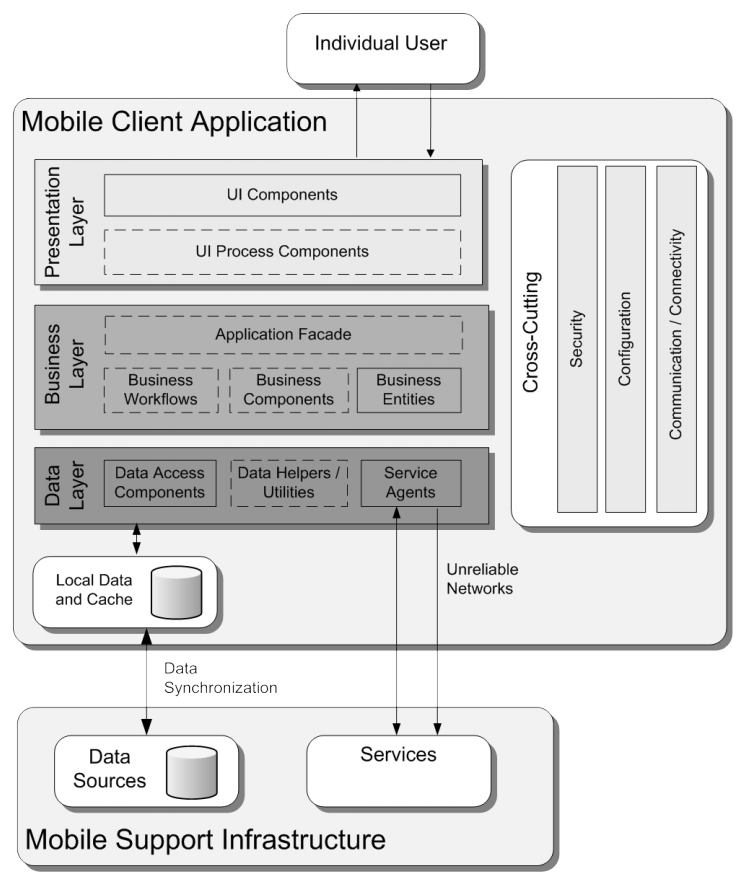
\includegraphics[width=0.6\textwidth]{imgs/mobileapparch.png}
  \caption[Arquitetura t\'ipica de uma  aplica\c c\~ao móvel]{Arquitetura t\'ipica de uma  aplica\c c\~ao móvel. \cite{mobileappbook}}
  
  \label{f:mobileapparch}
\end{figure}


No desenvolvimento de uma aplicação móvel tem que se ter em conta vários fatores importantes para garantir que a aplicação tem os requisitos necessários e é executável em qualquer smartphone. A lista de fatores a ter em conta é bastante alargada mas entre eles temos: Autenticação e Autorização, Armazenamento em Cache, Comunicação, Acesso de dados, Gestão de Exceções. \cite{mobileappbook}

\subsection{Autenticação e Autorização}

Uma estratégia de autenticação e autorização eficaz é importante para a segurança e fiabilidade de uma aplicação. Uma fraca autenticação pode deixar a aplicação vulnerável a uma utilização não autorizada. É necessário perceber que existe uma diferença entre autenticação e autorização. A autenticação é o processo de identificação de um utilizador com um identificador único e um elemento secreto (por exemplo uma palavra-passe). Um processo de autenticação garante, após o mesmo, que se trata de um utilizador específico. A autorização é o processo de controlo de ações sobre um serviço. Não indica um utilizador específico por si só. Para isto existe o protocolo de autorização OAuth que é um protocolo padrão para a autorização.\cite{oauth20}

\subsubsection{Protocolo de autorização OAuth}
O Open Authorization Protocol - OAuth é um protocolo de autorização que foi desenvolvido com o objetivo de solucionar os problemas relacionados com a gestão de identidades tal como Leiba \cite{leiba_oauth} referiu.
 A primeira versão é a 1.0 e foi lançada em 2007, e sua última revisão foi publicada em 2010, sendo especificada no \gls{RFC} 5849 \cite{oauth10}. Em 2012, a versão 2.0 do protocolo, OAuth 2.0, foi lançada com objetivo de resolver problemas encontrados
na versão 1.0, entre esses problemas tínhamos escalabilidade e complexidade \cite{oauth20}.
\par
Na versão 2.0 do protocolo são definidos quatro pontos de contacto necessários para a compreensão do fluxo de execução deste protocolo, são eles: Resource Owner - O proprietário do recurso, que é a entidade que tem o poder de conceder a permissão de acesso, aos seus recursos; Resource Server - O servidor de recursos, que é o responsável por guardar e responder às solicitações de acesso aos recursos protegidos, utilizando tokens de acesso; Client - Cliente, que é uma aplicação, que realiza solicitações de acesso aos recursos protegidos, ao servidor de recursos, em nome do proprietário, dono do recurso, após a obtenção de sua autorização; Authorization Server - O servidor de autorização, que é responsável por emitir tokens de acesso aos clientes, após autenticar e obter autorização do proprietário dos recursos \cite{oauth20}. Na figura seguinte é apresentado o fluxo do protocolo OAuth 2.0 mostrando a interação entre estes quatro pontos de contacto.

\begin{figure}[H]
  \centering
  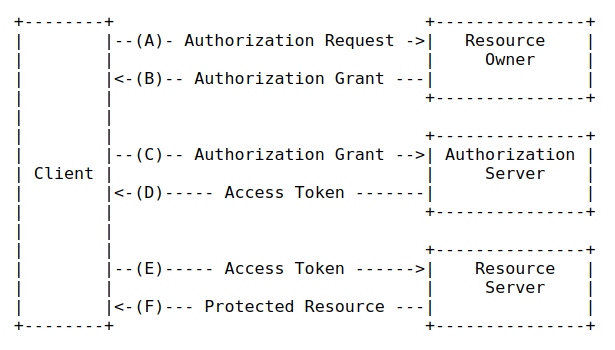
\includegraphics[width=0.8\textwidth]{imgs/oauth2flow.png}
  \caption[Fluxo do Protocolo 2.0]{Fluxo do Protocolo de autorização OAuth 2.0. \cite{oauth20}}
  \label{f:oauth2flow}
\end{figure}

\begin{enumerate}[label=(\Alph*)]
    \item O Client pede autorização ao Resource Owner para aceder aos seus recursos.
    \item Assumindo que o Resource Owner autoriza o acesso, o Client recebe um authorization grant (garantia de autorização). Essa credencial representa a autorização concedida pelo Resource Owner.
    \item O Client pede um access token ao Authorization Server, enviando o authorization grant.
    \item Assumindo que o Client foi autorizado com sucesso e que o authorization grant é válido, o Authorization Server gera um access token, sendo este enviado para o Client.
    \item O Client pede acesso a um recurso protegido pelo Resource Server, e autentica-se utilizando o access token.
    \item Assumindo que o access token é válido, o Resource Server responde ao pedido do Client enviando o recurso pedido.
\end{enumerate}

\subsection{Armazenamento em Cache}

A utilização da cache do dispositivo pode ser muito importante para aumentar o desempenho e a capacidade de resposta de uma aplicação. Quando não existe ligação à internet, a aplicação deve suportar a execução das operações principais, isto é, se uma aplicação tem como objetivo obter a frequência cardíaca de um paciente, é suposto se conseguir obter estes dados dos sensores mesmo sem estes poderem ser guardados no servidor, ou seja, podem ser guardados em cache até que se tenha possibilidade de fazer o envio para o servidor.
\par
Ao decidir os dados que podem ser guardados no dispositivo tem que se ter em atenção que os recursos são limitados, pois a memória de um smartphone não é como a de um computador.

\subsection{Comunicação do dispositivo}


A comunicação do dispositivo inclui a comunicação sem fios, comunicação com fios e ainda outro tipo de comunicação como por exemplo o Bluetooth. Na comunicação sem fios temos que ter em conta que temos que proteger os dados que estarão a ser transportados contra roubo ou adulteração. 
\par
Para comunicação entre dispositivos móveis e sensores será utilizada a tecnologia Bluetooth para cumprir o objetivo de selecionar os dispositivos e ler os dados recolhidos por estes.
A informação a ser recolhida tinha como foco o \gls{ECG} e a frequência cardíaca, como hipótese para isso tínhamos o \gls{VJ} que tem como funcionalidades ler o sinal \gls{ECG}, frequência cardíaca, nível bateria do dispositivo, etc.
A comunicação entre dispositivos móveis e backend será por Web services e para formato de dados será o JSON. Esta escolha foi feita pois desta maneira não vamos estar a limitar a plataforma que será protegida pelo protocolo de autorização OAuth. 

\subsubsection{Bluetooth}

Tal como nós pessoas comunicamos entre nós, os dispositivos móveis e os sensores também têm formas de se comunicar, como foco desta dissertação é receber dados de sensores para os guardar num backend capaz de agrupar estes dados corretamente, a tecnologia responsável por esta função será o Bluetooth.
Bluetooth é uma tecnologia criada em 1994 e foi concebida como uma alternativa sem fios para cabos de dados através da utilização de transmissões de rádio para conetar os dispositivos à distancia, e transferir dados entre eles. Esta tecnologia foi criada como um padrão aberto para permitir a conectividade e a colaboração entre diferentes produtos e indústrias \cite{bluetooth}.
Esta tecnologia está presente em grande percentagem de dispositivos eletrónicos vendidos atualmente, e quase todos os smartphones têm esta tecnologia.

\subsubsection{Vital Jacket}

O \gls{VJ} é um dispositivo médico que conjuga a tecnologia têxtil com soluções avançadas de engenharia biomédica, que permite uma monitorização contínua durante 72 horas seguidas. O dispositivo permite a configuração para adquirir diferentes sinais vitais tais como \gls{ECG}, frequência cardíaca, etc. É uma t-shirt confortável e fácil de vestir que vem equipada com um dispositivo que recolhe dados e os permite partilhar via Bluetooth em tempo real para os dispositivos móveis. \cite{vj}

\begin{figure}[H]
  \centering
  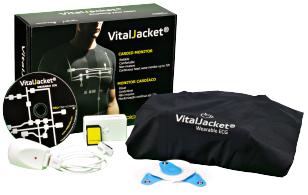
\includegraphics[width=0.6\textwidth]{imgs/vj.png}
  \caption[Kit VitalJacket]{Kit VitalJacket. \cite{vj}}
  \label{f:vjkit}
\end{figure}

\subsubsection{Web Services}

Os Web Services permitem que duas máquinas diferentes comuniquem entre si, ou que dois pedaços de código comuniquem entre eles. Para isto funcionar tem que existir um servidor que disponibilize uma \gls{API} que é um conjunto de métodos, e então os clientes podem chamar esses métodos e comunicar com o servidor pela internet por Web Services. Na próxima figura podemos ver uma troca de mensagens entre o cliente e o Web Service, em que um cliente envia uma mensagem de pedido a um Web Service, e recebe uma mensagem de resposta.



\begin{figure}[H]
  \centering
  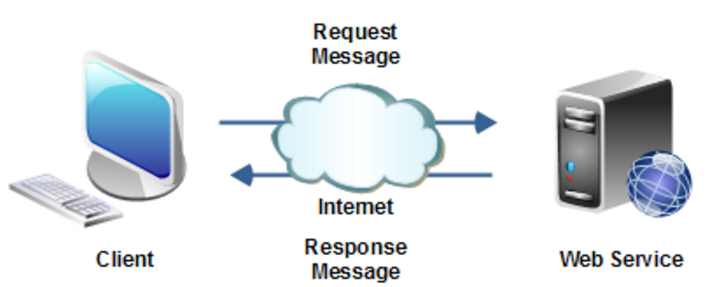
\includegraphics[width=0.6\textwidth]{imgs/wsscheme.png}
  \caption[Troca de Mensagens entre cliente e servidor]{Troca de Mensagens entre cliente e servidor \cite{wsjakob}}
  \label{f:wsscheme}
\end{figure}

Uma vantagem da utilização dos web services é que atualmente é uma tecnologia padrão, ou seja, é uma tecnologia que não é especifica de nenhuma linguagem de programação. O que acontece é uma interoperabilidade, apesar de os Web Services por exemplo serem desenvolvidos em Java, estes podem ser utilizados, ou seja, os pedidos podem ser efetuados através de um cliente que esteja a correr em Python.

Jakob Jenkov \cite{wsjakob} afirma que inicialmente o único formato de dados utilizado por um Web Service era apenas \gls{XML}, e só apenas
mais tarde foi permitido adicionalmente a utilização do \gls{HTML} e \gls{JSON} depois do aparecimento do \gls{REST}.

\subsubsection{ REST Web Services}

Segundo Elkstein\cite{whatisrest}, o \gls{REST} é um estilo de arquitetura que utiliza o \gls{HTTP} para fazer chamadas entre máquinas e tem como objetivo fundamental facultar serviços para ajudar no desenvolvimento de aplicações.

\gls{REST} caracteriza uma arquitetura centrada em recursos, especificando que cada recurso é identificado por um \gls{URI}, mediante o qual um conjunto de operações pode ser aplicado através de uma interface uniforme. Esta interface padrão uniforme para a comunicação entre servidores e clientes é o \gls{HTTP} e, em vez de declarar métodos, são aplicadas acções \gls{HTTP}, tais como POST, GET, PUT e DELETE. Estas quatro acções podem ser mapeadas para as acções típicas de dados \gls{CRUD}. A representação de cada recurso identificado por um URI, pode variar, podendo ser represendado em \gls{XML}, \gls{HTML}, \gls{JSON}, entre muitas outras possibilidades \cite{restwebservices}.


\subsubsection{JSON}

O \gls{JSON} é um formato de dados baseado em texto, é leve e utilizado para troca de informação independentemente da linguagem a ser utilizada. O \gls{JSON} é baseado em pares atributo-valor e a sua sintaxe é composta por quatro tipos de dados primitivos (strings, inteiros, booleans e null) e dois tipos estruturados (objetos e vetores) \cite{json}. 
\par
É um formato de dados  fácil de gerar, compreender e interpretar. Analisando código em \gls{JSON} é intuitivo associar a sua aparência, estrutura e sintaxe a muitas linguagens de programação existentes, razão pela qual foi facilmente adotada como uma alternativa ao \gls{XML} por parte de diversos programadores que viram no novo formato um modo mais natural e simples de definir dados.



\section{Arquitectura de uma aplica\c c\~ao mHealth}

Tipicamente a arquitetura das aplica\c c\~oes mHealth utiliza a Internet e Web Services para disponibilizar uma intera\c c\~ao entre os utentes e os m\'edicos \cite{mhealth}.
\par
Um m\'edico ou um utente pode facilmente aceder aos mesmos dados m\'edicos em qualquer momento e em qualquer lugar atrav\'es de dispositivos m\'oveis como computador, tablet ou smartphone. Para isto acontecer é necessário os dados estarem guardados num servidor para serem acedidos tanto pelos médicos como pelos utentes.

\begin{figure}[H]
  \centering
  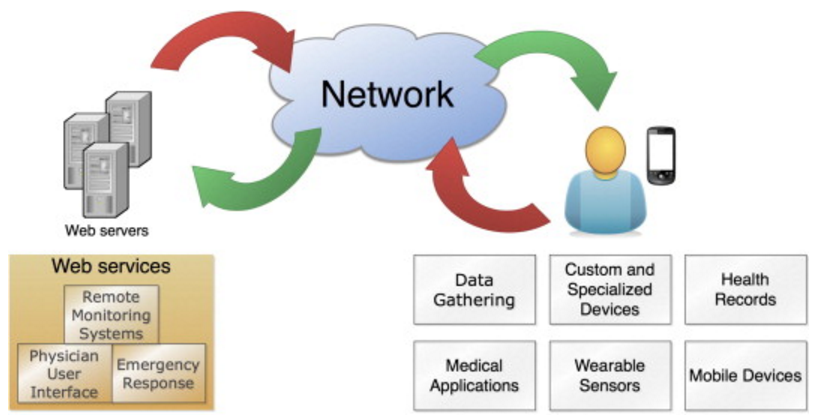
\includegraphics[width=0.7\textwidth]{imgs/mHealthArch.png}
  \caption[Arquitetura t\'ipica de uma  aplica\c c\~ao mHealth]{Arquitetura t\'ipica de uma  aplica\c c\~ao mHealth. \cite{mhealth}}
  
  \label{f:mhealtharch}
\end{figure}


\section{Desenvolvimento de uma aplica\c c\~ao mHealth}

Uma pesquisa desenvolvida pela PricewaterhouseCoopers descobriu que as solu\c c\~oes de mHealth que abrangem estes pr\'oximos seis princ\'ipios a seguir apresentados t\^em uma maior probabilidade de sucesso: Interoperabilidade, Integra\c c\~ao, Intelig\^encia, Socializa\c c\~ao, Resultados e Compromisso \cite{mhealthinsights}.
\par
Apesar das aplica\c c\~oes mHealth estarem numa crescente popularidade nos \'ultimos anos, muitas delas s\~ao rejeitadas ou n\~ao utilizadas pelo p\'ublico alvo pretendido, para contrariar esta realidade foi gerada uma discuss\~ao para se saber os requisitos e as considera\c c\~oes a ter durante e antes do desenvolvimento de uma aplica\c c\~ao mHealth.
\par
Depois deste estudo e discuss\~ao chegaram \`aa conclus\~ao que o desenvolvimento de uma aplica\c c\~ao deve estar dividida em 4 partes distintas constituindo uma pipeline de desenvolvimento, entre elas temos:  Prepara\c c\~ao, Desenvolvimento do Back-End, Desenvolvimento do Front-End e Lan\c camento da Aplica\c c\~ao\cite{mhealth-pipeline}.

\begin{figure}[!ht]
  \centering
  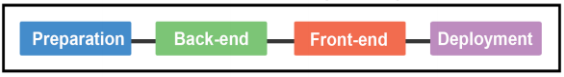
\includegraphics[width=0.9\textwidth]{imgs/mhealthDevPipeline.png}
  \caption[Esquema proposto para o desevolvimento de uma aplica\c c\~ao mHealth]{Esquema proposto para o desevolviment de uma aplica\c c\~ao mHealth. \cite{mhealth-pipeline}}
  
  \label{f:mhealthpipeline}
\end{figure}

\section{BackEnd para uma aplicação mHealth}

Para dar suporte à aplicação móvel é necessário a escolha de um backend robusto e seguro para que possamos lidar com dados e informações sensíveis e pessoais relacionados com o utente. Por isto deve se ter em atenção o envio, registo e armazenamento dos dados e informações no servidor. Para isso temos que ter em atenção algumas questões relacionadas com a segurança e privacidade dos dados. Vai ser agora apresentado algumas soluções possíveis.

\subsection{Open mHealth}

A \gls{OMH} foi fundada em 2011 e descreve-se a si própria como "uma start-up sem fins lucrativos que quebra as barreiras de integração trazendo significado aos dados clínicos digitais na área da saúde" \cite{omhabout}. A \gls{OMH} trabalha com especialistas da área da saúde e com programadores com o objetivo de tornar os dados de saúde digitais úteis e possíveis de utilizar em diversas plataformas. 
\par 
Um dos principais objetivos desta organização é que as aplicações na área da saúde não utilizem cada uma delas um formato de dados fechado e próprio, pois desta maneira os dados só são úteis dentro da própria aplicação, ou seja, estes não podem ser exportados para bases de dados de hospitais, ou clínicas, ou ainda outras aplicações na área da saúde. Podemos ver na figura seguinte a diferença que existe entre cada aplicação utilizar um formato de dados próprio, ou utilizar todas o mesmo formato\cite{omharticle}.

\begin{figure}[!ht]
  \centering
  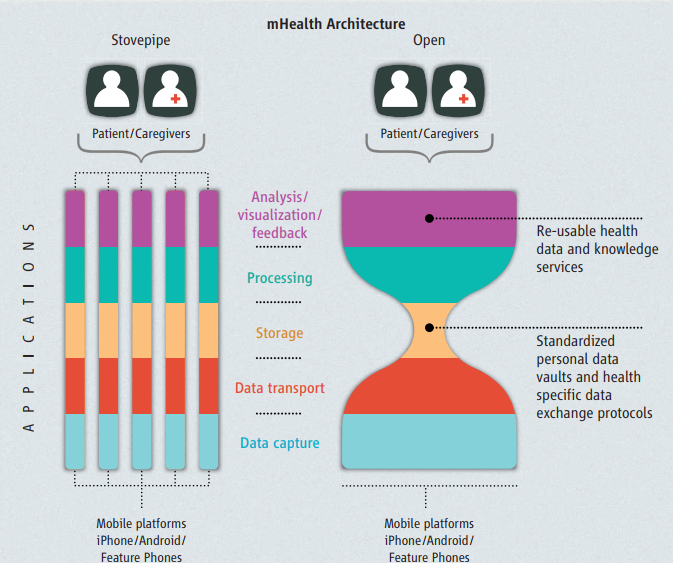
\includegraphics[width=0.9\textwidth]{imgs/openmharch.png}
  \caption[Arquitetura mHealth: Própria(''afunilada'') vs Open]{Arquitetura mHealth: Própria(''afunilada'') vs Open. \cite{omharticle}}
  
  \label{f:omharch}
\end{figure}

Através desta arquitetura podem ser partilhados diversos recursos entre as aplicações móveis na área da saúde, entre eles o mais importante é o modo e o local onde os dados são guardados, respeitando um padrão para o formato dos dados, ou seja, se duas aplicações diferentes forem guardar dados de um determinado tipo, como por exemplo frequência cardíaca, esses dados têm que respeitar um determinado formato, sendo estes guardados da mesma maneira independentemente da aplicação que o esteja a fazer.
\par 

A \gls{OMH} tem definido um conjunto de ''data schemas'' que é um conjunto de esquemas de dados criados e disponíveis que especificam um formato de dados para um determinado conteúdo como por exemplo a frequência cardíaca\cite{omhschemas}. Estes data schemas estão desenvolvidos em \gls{JSON} schema que serve para descrever um formato de dados, e os programadores têm que ter o cuidado de os datas schemas serem compatíveis com os \gls{JSON} schema associado. Na figura seguinte podemos ver exemplo de dados que é compativel com o \gls{JSON} schema associado que é a frequência cardíaca\cite{omhheartrate}.


\begin{figure}[H]
\inputminted{json}{code/heart-rate.json}
\caption[Exemplo de um \gls{JSON} compatível associado à frequência cardíaca]{Exemplo de um \gls{JSON} compatível associado à frequência cardíaca \cite{omhheartrate}}
\label{f:exemplo}
\end{figure}


Existe uma implementação de uma \gls{REST}full \gls{API} que suporta a criação, consulta e eliminação de dados inseridos. Esta \gls{API} permite a autorização utilizando o protocolo de autorização OAuth 2.0.

\subsection{FHIR}

Como vimos anteriormente para que os sistemas de serviços hospitalares comuniquem e partilhem  informação entre si, e com as plataformas online, é imperativo que compreendam o que está a ser comunicado.
\par 
Para compreenderem o que está a ser comunicado, os sistemas hospitalares e plataformas devem acordar na norma de comunicação. Existem várias normas para a troca de informação clínica. Existe uma norma que é o \gls{HL7} que é tipicamente utilizada em sistemas hospitalares \cite{whyihe} e tem ganho popularidade como uma norma flexível na troca de informação clínica estruturada.


Reconhecendo dos desafios da norma \gls{HL7}, a organização que definiu o \gls{HL7} desenvolveu a sua própria norma denominada de \gls{FHIR} \cite{hl7fhir}. O \gls{FHIR} consiste numa Framework normalizada com o objetivo de fornecer mecanismos de interoperabilidade para o \gls{HL7}, baseados nas tecnologias existentes na web, tais como \gls{XML}, \gls{JSON} , \gls{HTTP}, OAuth, entre outros \cite{hl7fhir}. Este suporta arquiteturas baseadas em \gls{REST}full e é suficientemente flexível para ser utilizado em diversos contextos, tais como aplicações mobile ou partilha de registos clínicos eletrónicos \cite{hl7fhir}.


\subsubsection{HL7}

A norma HL7 define uma Framework, e normas relacionadas, para troca, integração, partilha e requisição de  registos clínicos em formato eletrónico\cite{hl7}.
O HL7 encontra-se atualmente na sua versão 3\cite{corepointhealth}, mas a versão 2 do \gls{HL7} ainda é bastante utilizada, especialmente em sistemas antigos. 
\par
O problema que existia na versão 2 do \gls{HL7} é que cada sistema hospitalar ou clínica podia adaptar a norma à sua medida. O que acontece é que por exemplo, se formos desenvolver uma aplicação que comunica com vários  sistemas hospitalares ou clínicos, é necessário implementar uma interface especifica para cada um deles.
\par
Para resolver este problema saiu a versão 3, mas a sua adoção é cara e irá demorar bastante tempo \cite{corepointhealth}.

\subsection{GoogleFit}

O GoogleFit é uma aplicação móvel e uma \gls{API} \gls{REST} desenvolvido pela Google, na área do fitness. Permite aos utilizadores armazenar e aceder a informação relativa à sua condição física. Apesar de não ser desenvolvido com o objetivo de controlar os dados de saúde dos pacientes, pode ser visto como uma plataforma que cumpre alguns desses objetivos.
\par 
O GoogleFit é mais utilizado com o objetivo de monitorizar a condição física dos seus utilizadores, mas a Google permite o acesso aos dados recolhidos, através de \gls{API}’s criadas para esse efeito. Isto permite a criação de aplicações de saúde, visto que também é um dos objetivos da Google a integração de qualquer aparelho sensor. Resumindo, são dadas todas as ferramentas necessárias ao programador para aumentar o alcance da plataforma, permitindo-a ser utilizada com finalidades que a Google neste momento não cobre. 
De seguida mostro uma vista geral da plataforma GoogleFit.

\begin{figure}[!ht]
  \centering
  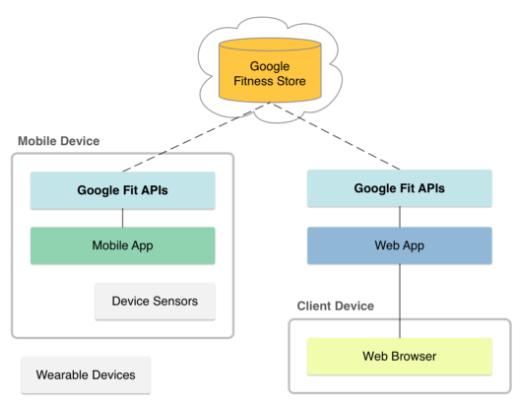
\includegraphics[width=0.9\textwidth]{imgs/googleFitOverview.PNG}
  \caption[Vista geral da plataforma GoogleFit]{Vista geral da plataforma GoogleFit \cite{googlefit}}
  
  \label{f:googleFitOverview}
\end{figure}

Como podemos perceber existe dois métodos principais de interagir com a plataforma. Através de uma aplicação para smartphones com o sistema operativo Android, desenvolvida também pela Google.  Também é possível a utilização de um website, que será um pouco mais limitado, mas se for apenas para visualizar os dados já inseridos na plataforma é bastante viável.

A \gls{API} \gls{REST} dá flexibilidade ao sistema. Com a utilização da \gls{API} passa a ser possível a criação de aplicações para outras plataformas que não o Android, tornando o Google Fit apelativo para um maior número de utilizadores. Esta \gls{API} está protegida pelo protocolo de autorização OAuth 2.0 e utiliza para formato dos dados \gls{JSON}\cite{googlegetstarted}. 

\section{Análise Comparativa}

\begin{table}[H]
\centering

\label{tabelaComparativa}
\begin{tabular}{|>{\columncolor[HTML]{C0C0C0}}c |c|c|c|c|c|c|}
\hline
\textbf{\backslashbox{Requisito}{Plataforma}}                                                                        & \cellcolor[HTML]{C0C0C0}\textbf{OMH} & \cellcolor[HTML]{C0C0C0}\textbf{FHIR} & \cellcolor[HTML]{C0C0C0}\textbf{\begin{tabular}[c]{@{}c@{}}Google\\ Fit\end{tabular}} & \cellcolor[HTML]{C0C0C0}\textbf{\begin{tabular}[c]{@{}c@{}}Health\\ Vault\end{tabular}} & \cellcolor[HTML]{C0C0C0}\textbf{\begin{tabular}[c]{@{}c@{}}Apple\\ Research\\ Kit\end{tabular}} & \cellcolor[HTML]{C0C0C0}\textbf{\begin{tabular}[c]{@{}c@{}}Research\\ Stack\end{tabular}} \\ \hline

\textbf{Dados do Paciente} & - & X & - & X & X & X \\ \hline
\textbf{\begin{tabular}[c]{@{}c@{}}Facilidade de \\ Desenvolvimento\end{tabular}} & X & - & X & - & - & - \\ \hline
\textbf{\begin{tabular}[c]{@{}c@{}}Modelo de Dados \\ Normalizado\end{tabular}} & X & X & - & - & - & - \\ \hline
\textbf{\begin{tabular}[c]{@{}c@{}}Extensibilidade do \\ Modelo de Dados\end{tabular}} & X & - & X & - & - & - \\ \hline
\textbf{Interoperável} & X & X & - & - & - & - \\ \hline
\textbf{Segurança e Privacidade} & X & X & X & X & & \\ \hline
\textbf{MultiPlataforma} & X & X & X & & & \\ \hline
\end{tabular}
\caption{Comparação dos diferentes backends}
\end{table}

Depois de analisados três serviços de backend para dar suporte a uma aplicação móvel na àrea de saúde, faz-se aqui uma breve analise comparativa das suas características. Cada um apresenta vantagens nuns aspetos e desvantagens noutros.
\par 
A complexidade do \gls{FHIR} é bastante grande, tornando-o bastante completo, a grande desvantagem deste backend é não ser possível extender os dados. Tendo em conta que um dos objetivos seria também ler, guardar e visualizar \gls{ECG}, este backend fica a perder, apesar da grande variedade dos tipos de dados existentes este não é contemplado.
\par 
Em relação ao GoogleFit tem uma boa \gls{API} \gls{REST}, apesar de não haver nenhum tipo dados onde se pudesse guardar os dados do paciente a extensibilidade do modelo de dados é possível. O modelo de dados é extensível mas existe uma limitação quanto ao modelo de dados, apenas podem ser utilizados como tipo de dados o int e o float, ou seja, não existe o tipo objeto e array.
\par 
O \gls{OMH} tem uma \gls{API} \gls{REST}, também como o GoogleFit não tem a possibilidade de guardar dados do Paciente, mas o modelo de dados é também extensível. A grande vantagem que tem é um conjunto de \gls{JSON} Schemas definidos que podem ser utilizados para validar a entrada dos dados no backend. Deste modo nenhum tipo de dados vai ser inserido se não respeitar as devidas definições. Ao criarmos novos \gls{JSON} schemas podemos reutilizar os já existentes para definir determinados atributos, o que torna tudo bastante mais fácil

\chapter{ novo Capítulo}


\section{OMH}

\subsection{Criar um novo tipo de dados}
A criação de um novo tipo de dados pode ser feita com a ajuda do repositório ''schemas'' \cite{schemas-rep} que foi criado pela organização da \gls{OMH}. Para isto vai necessitar de algumas ferramentas entre elas: o git \cite{git-install} para puxar o repositório; o Java 8 \cite{java-overview} para executar o validador; um editor de texto como por exemplo o atom \cite{atom-install}. Vou descrever agora a lista de tarefas para conseguir efetuar a criação de um novo tipo de dados. Para este tutorial vou criar o tipo de dados acelerómetro. É um dos tipos de dados que são obtidos através do \gls{VJ}.

\begin{enumerate}
  \item Clonar o repositório correspondente para um diretório à sua escolha com o comando \par
  ''git clone https://github.com/openmhealth/schemas'' 
  De seguida vamos fazer duas coisas principais: uma delas é criar o ficheiro que define o novo tipo de dados; a outra é criar um ficheiro com uma amostra do novo tipo de dados.
  \item Criar um ficheiro que define o tipo de dados em \gls{JSON} schema, para isso, adicione um novo ficheiro no diretório schema/omh. O nome deste ficheiro tem que ser composto pelo nome que quer dar ao tipo de dados e a versão correspondente, tem que terminar com a extensão .json. No meu caso criei com o nome accelerometer-1.0.json  \par A versão escolhida aqui é a 1.0 mas podia ser qualquer outra. Pode reparar que no diretório schema/omh tem acesso a todos os ficheiros que definem todos os tipos de dados.
  \item Adicionar uma nova pasta ao diretório testdata/omh como o nome respetivo ao ficheiro criado anteriormente. Neste caso criar uma pasta com o nome accelerometer.
  \item Vai agora criar uma pasta correspondente à versão introduzida no ponto 2. Neste caso é 1.0 e uma outra pasta dentro da criada anteriormente com o nome shouldPass.
  \item Dentro do diretório shouldPass vai ter que criar um ou vários ficheiros para ser utilizados como amostras do tipo de dados. O objetivo deste diretório é ter várias amostras válidas testando-as com o tipo de dados criado no ponto 2. Para este tutorial criei o ficheiro example.json. \par Neste ponto o nome do ficheiro é opcional só tem que acabar com a extensão .json
  Como criou o diretório shouldPass, pode também criar o diretório shouldFail criando também vários ficheiros para testar o tipo de dados criado. \par 
  Neste ponto tem tudo preparado para começar a criar o novo tipo de dados e validar a amostra com a nova definição do novo tipo de dados criados
  
  \begin{figure}[!ht]
  \centering
  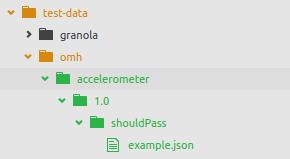
\includegraphics[width=0.5\textwidth]{imgs/newsampledata.png}
  \caption[Esquema de diretório para o novo sample]{Esquema de diretório para o exemplo do novo tipo de dados}
  
  \label{f:directorynewsample}
\end{figure}
  
\item Vamos agora preencher o ficheiro com a definição do novo tipo de dados, aquele que criou no ponto 2. O ficheiro vai ser criado no formato de \gls{JSON} schema. Para suportar a criação deste ficheiro pode reutilizar schemas existentes \cite{schema-library} e referênciá-los, deste modo estará a criar um modelo com tipos de dados normalizados. No meu caso vou reutilizar um schema para definir a data/hora e um outro para definir o tipo de atividade que está a efetuar no momento da leitura. Os restantes dados estão relacionados com o acelerómetro em si, a sessão e a leitura respetiva.
O ficheiro fica do seguinte modo: 

\begin{figure}[H]
\inputminted{json}{code/accelerometer-1.0.json}
\caption[\gls{JSON} schema para o novo tipo de dados de acelerómetro]{\gls{JSON} schema para o novo tipo de dados de acelerómetro}
\label{f:accelerometer-json-schema}
\end{figure}

\item Preencha o ficheiro com uma amostra do novo tipo de dados, para isso tem que ter em conta a definição utilizada, pois porque se esta amostra não for compatível não vai passar no validador.

\begin{figure}[H]
\inputminted{json}{code/example.json}
\caption[Exemplo do tipo de dados de acelerómetro]{Exemplo do tipo de dados de acelerómetro}
\label{f:accelerometer-json-data}
\end{figure}

\item Para compilar e executar o validador tem que executar o comando ''./gradlew test-data-validator:bootRun'' no diretório principal ''schemas'' ou então execute o comando ''./gradlew bootRun'' no diretório ''schemas/test-data-validator''. 


\end{enumerate}

\chapter{Conclus\~ oes}

Que conclus\~oes?

%
% The bibliography
%
\cleardoublepage

\renewcommand{\bibname}{Lista de Referências}
\bibliography{references}

\cleardoublepage

\end{document}
